\documentclass[12pt]{article}
\usepackage{setspace}
\usepackage[utf8]{inputenc}
\usepackage[a4paper,top=20mm]{geometry}
\usepackage{hyperref}
\usepackage{amsfonts}
\usepackage{mathdots}
\usepackage{graphics}
\usepackage{tikz}
\graphicspath{ {./images/} }
\usepackage{graphicx}
\usepackage{amssymb}
\usepackage{amsmath}
\usepackage{parskip}
\usepackage{pifont}
\newcommand{\floor}[1]{\left\lfloor #1 \right\rfloor}
\newcommand{\ceil}[1]{\left\lceil #1 \right\rceil}
\newcommand\ddfrac[2]{\frac{\displaystyle #1}{\displaystyle #2}}
\newcommand*\circled[1]{\tikz[baseline=(char.base)]{
            \node[shape=circle,draw,inner sep=2pt] (char) {#1};}}
\title{Speed Proving Tournament 14 Questions}
\author{Bikramjyot, Farhan, Himanshu, Ishaan, Rachit}
\begin{document}
\doublespacing
\maketitle

\section{GEOMETRY}

% \begin{enumerate}
    If four different points $A, B, C, D$ lie on a circle satisfying the following conditions:
\begin{itemize}
  \item $\vec{|AB|} = 8$
  \item $\vec{AC} \cdot \vec{AB} = 0$
  \item $\vec{AD} = \frac{1}{2} \vec{AB} - 2 \vec{BC}$
\end{itemize}
What is the value of $\vec{|AD|}^2$
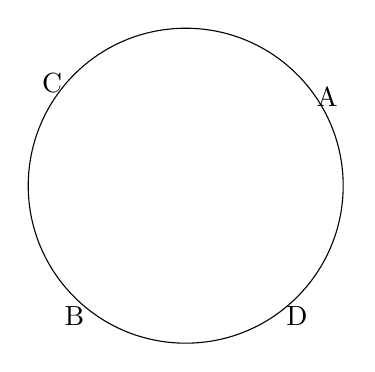
\begin{tikzpicture}

% Define the circle
\draw (0,0) circle [radius=2];

% Place points A, B, C, and D on the circle
\coordinate[label=above:A] (A) at (26:2);
\coordinate[label=above:C] (B) at (148:2);
\coordinate[label=below:B] (C) at (225:2);
\coordinate[label=below:D] (D) at (315:2);


\end{tikzpicture}

% \end{enumerate}

\section{ALGEBRA}

\begin{enumerate}
    \item $P(x)$ is a 4th degree polynomial with real coefficients such that $P(x) \geq x$.
    $P(1) = 1$, $P(2) = 4$, $P(3) = 3$.
    Find the value of $P(4)$
    \item $8a^ab^b = 27a^bb^a$. 
    Find the value of $a^2 + b^2$.
    \item Let $a,b,c$ be positive real numbers such that 
    \begin{align*}
        \frac{a}{1+b} + \frac{b}{1+c} + \frac{c}{1+a} = 1
    \end{align*}
    Prove that $abc \leq \frac{1}{8}$
\end{enumerate}

\section{NUMBER THEORY}
\begin{enumerate}
    \item Prove that for \(n \geq 2\), \(\sqrt[n]{n}\) is irrational.
    \item Prove that the sum of reciprocals of the first \(n\) triangular numbers is less than 2.
    \item The Euler's totient function of $n$, $\phi(n)$, is defined as the number of positive integers upto $n$ which are relatively prime to $n$. Find the positive integer $\leq 1000000$ such that $\frac{n}{\phi(n)}$ is maximum.
\end{enumerate}
    Old questions

\begin{enumerate}
    \item Let $d$ be any positive integer not equal to 2, 5 or 13, show that we can always choose any two distinct numbers $a$ and $b$ from $\{2,5,13,d\}$ such that $ab-1$
    \item Show that $4^{n}+n^{4}$ is composite for all integers $n\ge 2$       
    \item Prove that if the number of factors of 2 in $n!$ is $n-1$, then $n$ is a power of 2
    \item Prove that for every prime $p$, you can construct a number having sum of digits $p$ that is divisible by $p$
    \item Prove that if seven distinct numbers are selected from $\{1, 2,\dots, 11\}$, then some two of these numbers sum to 12.
\end{enumerate}

\section{PIGEONHOLE PRINCIPLE}
\begin{enumerate}
    \item A chess master who has 11 weeks to prepare for a tournament decides to play at least one game every day, but, in order not to tire himself, he decides not to play more than 12 games during any calendar week. Show that there exists a succession of consecutive days during which the chess master will have played exactly 21 games.
    \item Given any set of $n$ integers $a_1, a_2, \cdots, a_n$, prove that there must exist $0 \leq k < l \leq n$ such that $\sum_{j=k+1}^{l}a_j$ is divisible by $n$.

\end{enumerate}
Old questions
\begin{enumerate}
    \item For $n>1$, consider an n × n chessboard and place pieces at the centres of different squares. With 2n chess pieces on the board, show that four pieces among them form the vertices of a parallelogram
    \item Prove that every convex polygon with an even number of sides has a diagonal that is not parallel to any of its sides
    \item The set $\{1,2,3,\dots,16\}$ is partitioned into three sets. Prove that one of the subsets contains some numbers $x$, $y$, and $z$ (not necessarily distinct) such that $x+y=z$.
\end{enumerate}

\section{SEQUENCES}
Old questions
\begin{enumerate}
    \item For an infinite sequence $<a_{ij}>$, $\displaystyle\sum_{i=1}^{\infty}\sum_{j=1}^{\infty} a_{ij}$ is not always equal to $\displaystyle\sum_{j=1}^{\infty}\sum_{i=1}^{\infty} a_{ij}$
    \item A sequence of positive integers $<a_{n}>$ is defined as follows. $a_{1}$ is an arbitrary positive integer, and for $n \ge 1$, $a_{n+1}=a_{n}/5$ if $a_{n}$ is divisible by 5, and $a_{n+1} = \floor{a_{n}\sqrt{5}}$ if $a_{n}$ is not divisible by 5. Prove that eventually, the sequence will be strictly increasing
    \item Given are the positive integers $a_{0},\dots,a_{100}$ such that $a_{1} > a_{0}$, $a_{2} = 3a_{1} - 2a_{0}$, $a_{3} = 3a_{2} - 2a_{1}$,$\dots$,$a_{100} = 3a_{99} - 2a_{98}$. Prove that $a_{100} > 299$.

\end{enumerate}

\section{COMBINATORICS}
\begin{enumerate}
    \item Give a \textbf{combinatorial} proof that 
    \begin{align*}
    (n-k)\binom{n}{k} = n\binom{n-1}{k}
    \end{align*}
    (Note to self: no algebraic proofs allowed)
    \item How many bit strings of length 10 contain either five consecutive 0s or five consecutive 1s?
    \item Find the number of ways to tile a $2 \times n$ grid with $l \times k$-sized rectangles $(l \leq 2)$ (you may leave the answer in terms of matrices and determinants).
\end{enumerate}



\section{MISCELLANEOUS}
\begin{enumerate}
\item You pick up a meter stick with 100 ants on it. Each ant walks \(1 \, \text{cm/s}\) toward an end of the stick, and it reverses direction any time it encounters another ant. Prove that after \(100\) seconds, all ants have fallen off the stick.

\end{enumerate}
Old questions
    
\begin{enumerate}
    \item Let $ABCD$ be a quadrilateral with an inscribed circle. Prove that $AB+CD=AD+BC$
    \item Prove that for positive integers $a$,$b$ and $c$, $\frac{b}{a+c} + \frac{c}{b+a} + \frac{a}{c+b} \geq \frac{3}{2}$
    \item For any quadrilateral with sides $a$, $b$, $c$ and $d$, $\frac{a^{2}+b^{2}+c^{2}}{d^{2}} \geq \frac{1}{3}$
    \item Prove that every convex polyhedron has at least two faces with the same number of sides.

\end{enumerate}
\pagebreak

\end{document}